%%%%%%%%%%%%%%%%%%%% author.tex %%%%%%%%%%%%%%%%%%%%%%%%%%%%%%%%%%%
%
%%%%%%%%%%%%%%%% Springer %%%%%%%%%%%%%%%%%%%%%%%%%%%%%%%%%%

\title*{A detailed analysis of a GP run}
% Use \titlerunning{Short Title} for an abbreviated version of
% your contribution title if the original one is too long
\author{Nicholas Freitag McPhee, Maggie M. Casale, Mitchell Finzel, Thomas Helmuth and Lee Spector}
\authorrunning{McPhee, Casale, Finzel, Helmuth, and Spector}
% Use \authorrunning{Short Title} for an abbreviated version of
% your contribution title if the original one is too long
\institute{Nicholas Freitag McPhee, Maggie M. Casale and Mitchell Finzel \at University of Minnesota, Morris; Morris, MN USA
\and Thomas Helmuth \at Washington and Lee University, Lexington, VA USA
\and Lee Spector \at Hampshire College, Amerherst, MA USA}

\maketitle

\abstract{We analyze the key events in a GP run!}

\begin{keywords}
	genetic programming, PushGP, ancestry graph, lineage, inheritance
\end{keywords}
\index{genetic programming}
\index{PushGP}
\index{ancestry graph}
\index{lineage}
\index{inheritance}
\\
\section{Introduction}
\label{sec:introduction}

Motivate the work!

\section{Plush genomes and PushGP operators}
\label{sec:background}

The run presented here uses the PushGP genetic programming system, which evolves programs in the Push programming language \citep{spector:2002:GPEM, 1068292}. Push programs use multiple typed stacks to store and manipulate data. Instructions take their arguments from stacks of the appropriate types and they leave their results the appropriate stacks. Push provides support for iteration, recursion, conditional execution, and automatically-defined subroutines through runtime code manipulation, making it a Turing-complete language \citep{1068292}. PushGP implementations have been written in Clojure, C++, Java, JavaScript, Python, and others. Many of these are available from the Push project page.\footnote{\url{http://pushlanguage.org/}} The run presented here was conducted using the Clojure implementation of PushGP\footnote{Clojush: \url{https://github.com/lspector/Clojush}}.

Push gains much of its power as an evolutionary language from its ability to manipulate code, including the currently executing code, as a program runs. The running program is stored on the \textit{exec} stack, allowing instructions to change code before it runs. Push programs are hierarchically structured into code blocks delimited by parentheses. Each code block acts as a single unit when code manipulating instructions act on them. For example, the \texttt{exec\_if} instruction deletes the second code block on the \texttt{exec} stack if the top item on the \texttt{boolean} stack is true, and deletes the first code block on the \texttt{exec} stack if it is false.

Unlike previous versions of PushGP, Clojush has recently changed to not evolve Push programs directly, but instead uses a new linear genome representation \citep{Helmuth:2016:GPTP}. Each \textit{Plush genome}\footnote{\textbf{L}inear \textbf{Push}} consists of a linear sequence of instructions (including literals), and is translated into a Push program prior to execution. Each instruction may have one or more epistatic markers attached that modify how the genome is translated into a Push program.
%For example, the \textit{silent} marker is a boolean that tells whether a particular instruction will appear in the translated program. 

Most relevant to this study is the \textit{close} epistatic marker, which affects the hierarchical composition of programs. Since many Push instructions do not take arguments, as in code blocks, from the \textit{exec} stack, it makes sense to limit the appearance of code blocks to follow only instructions that make use of them. Each instruction that takes one or more argument from the \textit{exec} stack automatically opens one or more code blocks. Then, the integer close marker attached to each instruction tells how many opened code blocks to close after the instruction. During translation from Plush genome to Push program, an open parenthesis is placed after each instruction that requires a code block, and a matching closing parenthesis is placed after a later instruction with a non-zero close marker. These code blocks can create hierarchically nested Push programs, allowing, for example, structures such as nested looping and subroutines containing conditional code.

The use of linear genomes allows PushGP to use simple uniform genetic operators. The operators used in this study are inspired by the operator ULTRA. ULTRA, designed for use on Push programs, requires programs to be translated into a linear form and back \citep{Spector:2013:GPTP}, potentially requiring repair of the program. Our main crossover operator, \textit{alternation}, traverses two parents in parallel while copying instructions from one parent or the other to the child.
%While traversing the parents, copying can jump from one parent to the other with probability specified by the \textit{alternation rate} parameter. When alternating between parents, the index at which to continue copying may be offset backward or forward some amount based on a random sample from a normal distribution with mean 0 and standard deviation set by the \textit{alignment deviation} parameter.
We also use a \textit{uniform mutation} operator that traverses a parent, replacing each instruction with some small probability. Similarly, a \textit{uniform close mutation} operator can change the close epistatic marker attached to an instruction by incrementing or decrementing it. Finally, we often apply an alternation operator followed by a uniform mutation of the result, inspired by the ULTRA operator \citep{Spector:2013:GPTP}.

Push implements a method of automatic simplification, which takes a program and converts it into a smaller, semantically equivalent program. This process uses hill-climbing to remove instructions and code blocks from the program, checking at each step that the resulting program produces the same error vector as the original program \citep{Spector:2014:GECCOcomp}.


%\subsection{THIS COPIED FROM TOM'S THESIS}

%% I (Tom) left the following in the tex in case we need more info later; most of it isn't represented above. If we use it, it shouldn't be copied directly as to not plagiarize Tom's thesis.

% Push dedicates a separate stack for each data type. Instructions take their arguments from stacks of the appropriate types and they leave their results on stacks of the appropriate types. This allows instructions and literals to be freely intermixed regardless of type while still ensuring execution safety. The convention in Push regarding instructions that are executed in contexts that provide insufficient arguments on the relevant stacks is that these instructions act as ``no-ops''; that is, they do nothing.

%Push traditionally takes results from the top items on stacks after executing a program. For example, a program that returns an integer will take the top value on the integer stack as its output. This convention means that some evolved programs might not return a value of the correct type, if the relevant stack is empty following execution; in this scenario, we penalize the program for failing to return a result. Push also has the ability to print literals to standard output; in our implementation this simply concatenates printed material to a string of whatever has been printed so far, but this could easily be changed to print to standard output.


\section{Analysis of a run}


Our goal here is to give a deep analysis of a single run of PushGP, exploring and analyzing many of the programs, selections, and variations that make up this run. We chose to analyze a run on the Replace Space With Newline (RSWN) problem, taken from a recent general program synthesis benchmark suite \citep{Helmuth:2015:GECCO}. In this problem, a program is given a string as input and should perform two tasks: first, it must print the result of replacing each space in the input with a newline character, and second, it must functionally return the number of non-whitespace characters in the input. Push functionally returns values by taking them from the top of relevant stacks. For example, each program evolved in this run returns the top integer on the integer stack as its output, unless the stack is empty. We include instructions that allow programs to print literals to standard output.


\begin{itemize}
	\item Describe the basics of the run (length, etc.).
\end{itemize}

Then work backwards from the winner back through to the start of the run.

\subsection{Full ancestry graph}

Figure~\ref{fig:run0Labelled} shows the full ancestry tree of the 13 successful 
individuals in this run. Each individual in the run is represented with a
rectangle containing an identifier of the form \texttt{X:Y}, where \texttt{X}
is the generation number, and \texttt{Y} is an arbitrary individual number
within that generation. Each generation is a row, with the initial random
individuals being at the top and the 13 successful individuals at the bottom.

\begin{sidewaysfigure}[tb!p] %[b] sets the image at the bottom of the page; t = top, b = bottom, h = here%
	% \sidecaption
	% Use the relevant command for your figure-insertion program
	% to insert the figure file.
	% For example, with the graphicx style use
	\begin{center}
		\vspace{0.6\columnwidth}
		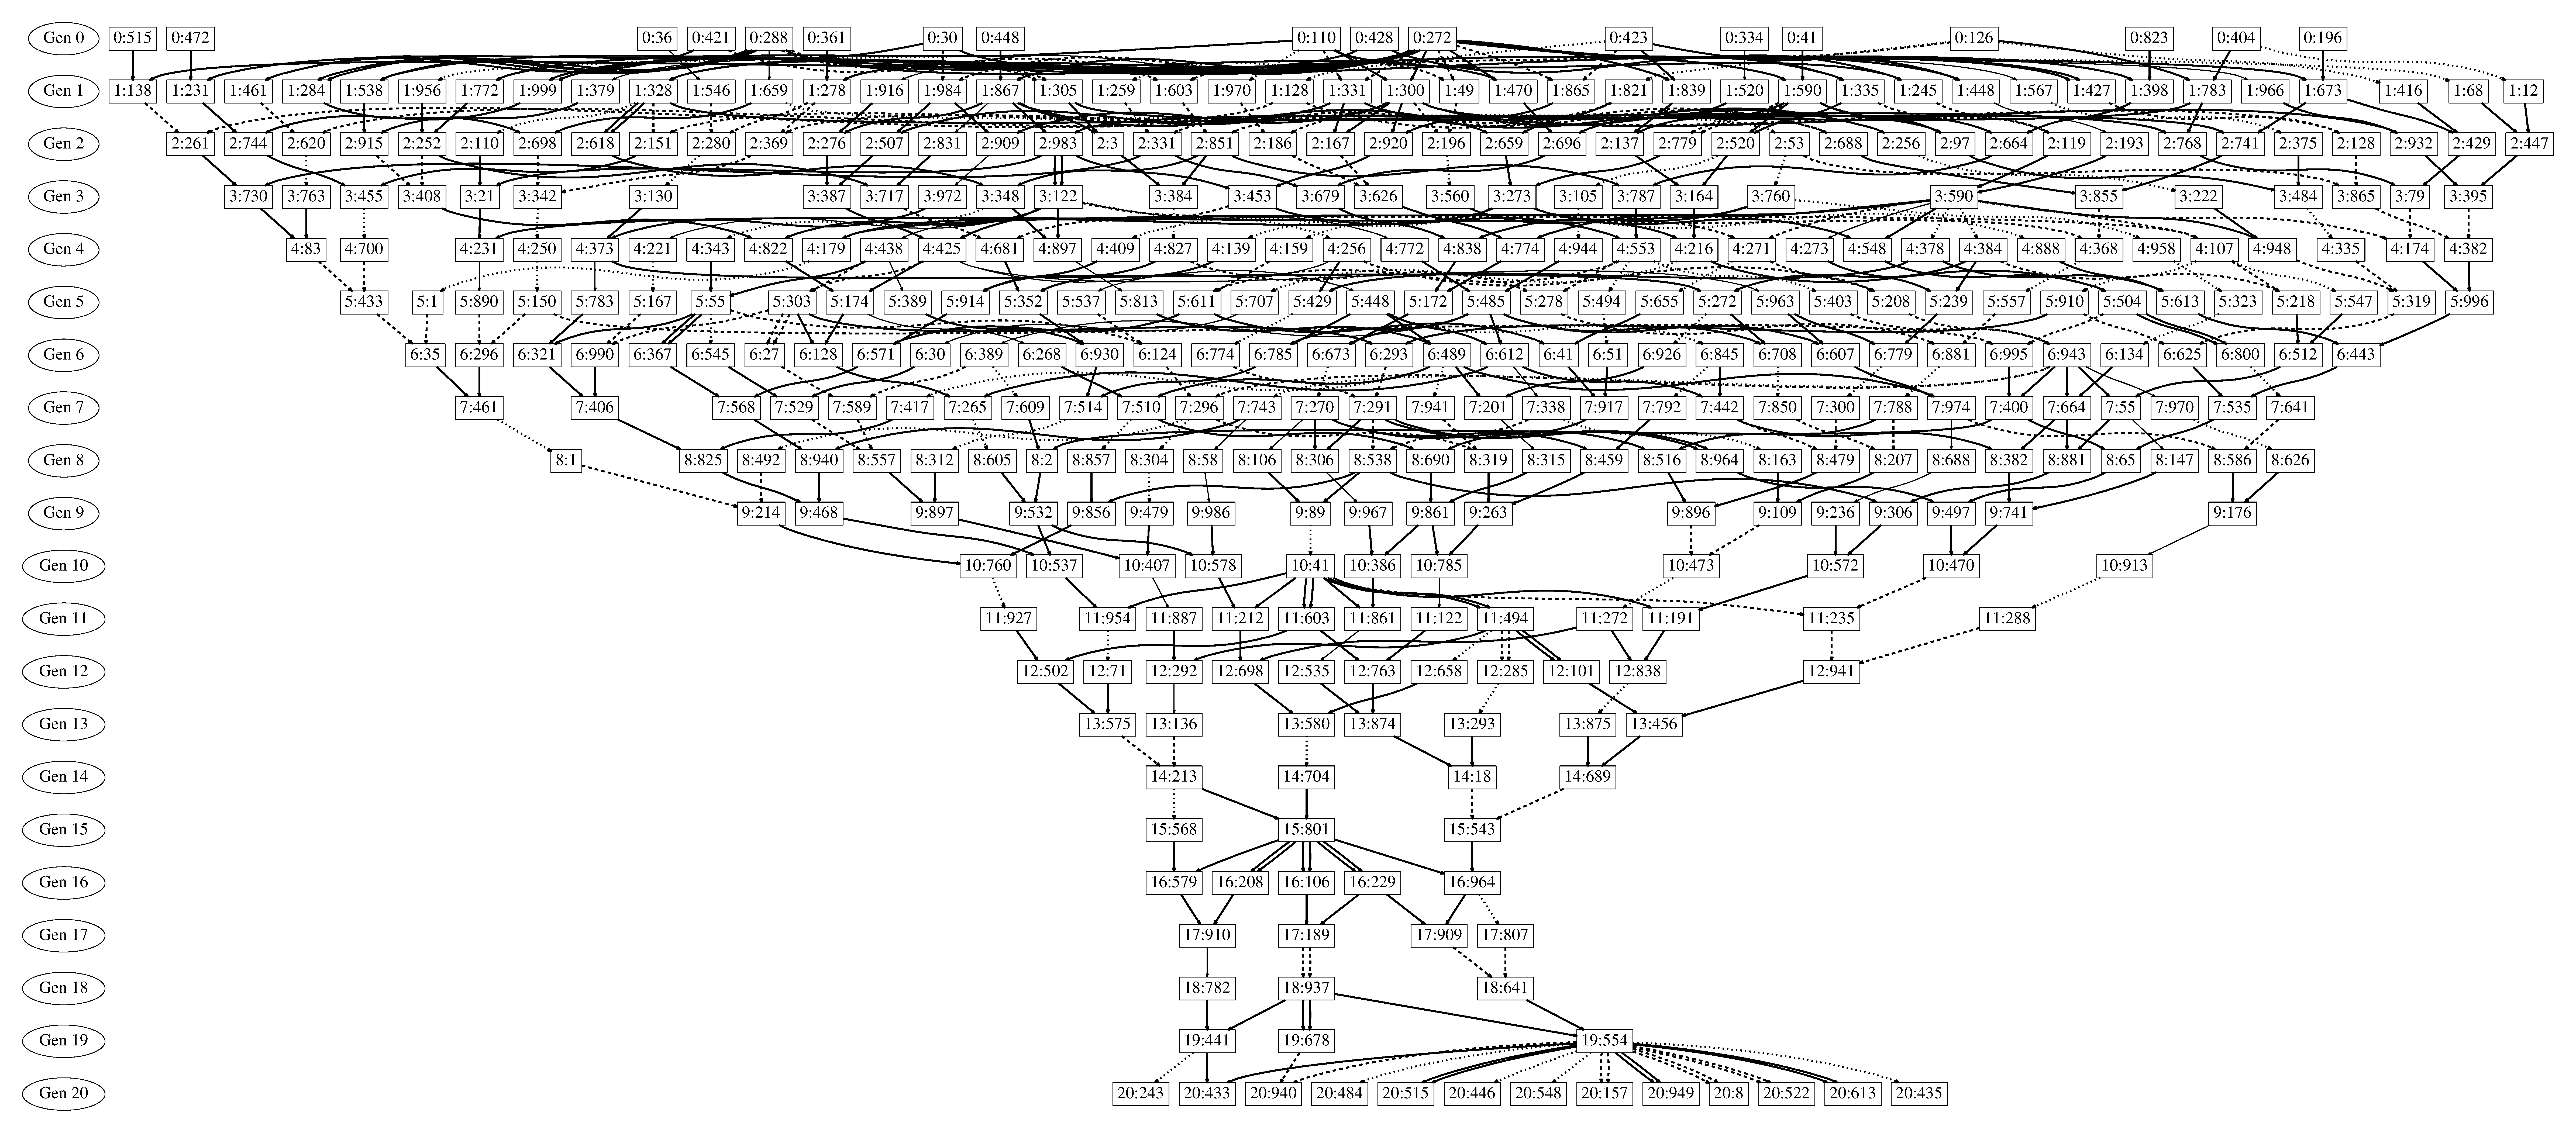
\includegraphics[width=\columnwidth]{../figures/run0_GPTP_2_font_30}
	\end{center}
	\caption{The labelled run.}
	\label{fig:run0Labelled}       % Give a unique label
\end{sidewaysfigure}

The edges indicate the particular genetic operator used to construct a child
as follows:
\begin{itemize}
	\item Thick black lines: alternation and uniform mutation
	\item Dashed: alternation
	\item Dotted: uniform mutation
	\item Thin black lines: uniform close mutation
\end{itemize}

This graph includes \emph{every} individual in this run that was an 
ancestor of one of the winners, i.e., every individual that could possibly have 
contributed genetic material to one of the winners. Note, however, that not
all these individuals actually contributed any genetic material to those
solutions. There are, for example, cases where one of the parents actually
contributed no material in a recombination (alternation) event, and cases where
a parent did contribute some genetic material, but that material was later
removed or replaced in subsequent mutations or recombinations. 

Conversely, while the individuals not represented in this graph are
guaranteed to have not contributed to the genetics of the successful
individual, they might have still had some substantial impact on the
run's overall dynamics. The presence of those individuals and their
error vectors could certainly affect lexicase selection's choice of parents,
for example, which could substantially impact the dynamics.

\subsection{Filtered ancestry graph}

Despite the short length of this run, and the restriction to just displaying
ancestors of successful individuals, Figure~\ref{fig:run0Labelled} still
contains 394 nodes and 629 edges, making it difficult to analyze in full.
Figure~\ref{fig:run0Filtered} is a version of the same graph that further
filters the ancestry tree, attempting the highlight the individuals that
are most likely to have contributed a significant amount of genetic material
to the solutions.

\begin{figure}[tb!p] %[b] sets the image at the bottom of the page; t = top, b = bottom, h = here%
	% \sidecaption
	% Use the relevant command for your figure-insertion program
	% to insert the figure file.
	% For example, with the graphicx style use
	\begin{center}
		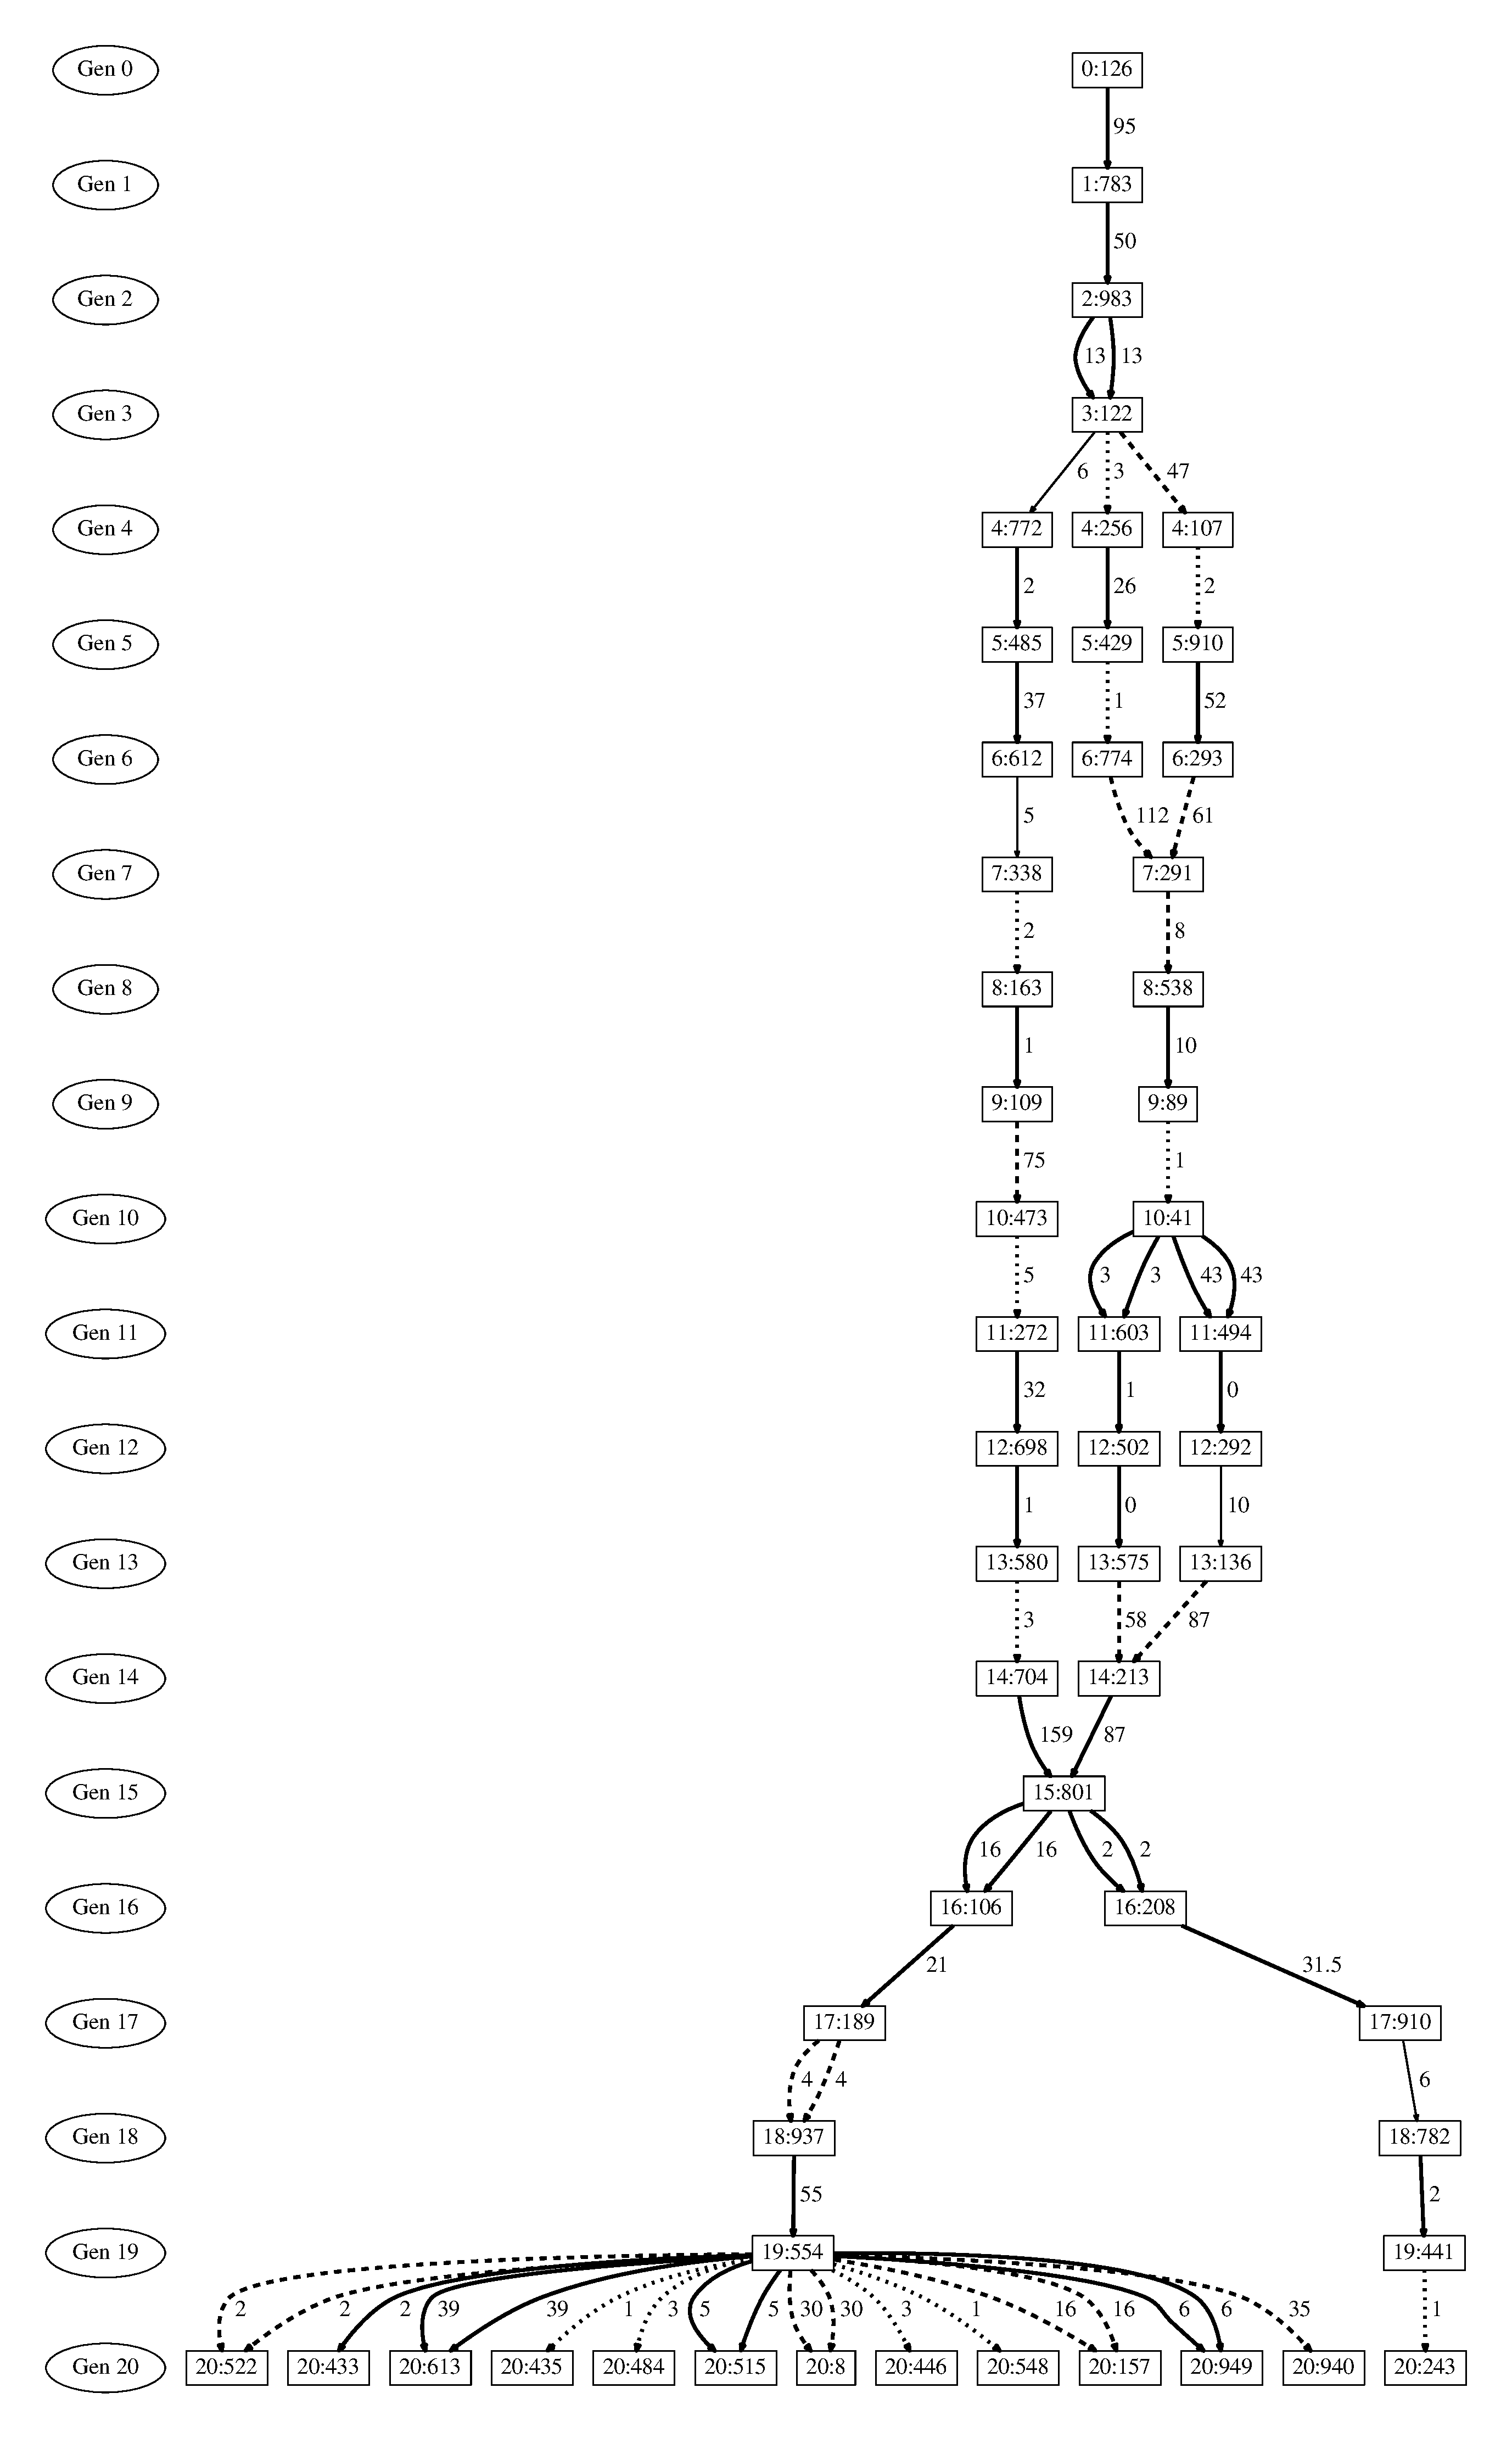
\includegraphics[width=0.9\textwidth]{../figures/run0_GPTP_filtered}
	\end{center}
	\caption{The filtered version of the run's ancestry graph.}
	\label{fig:run0Filtered}       % Give a unique label
\end{figure}

We implemented this filtering by first computing the Damerau-Levenshtein 
distance (DL-distance)
between genome vectors for each parent-child pair; these distances
are indicated as edge labels in Figure~\ref{fig:run0Filtered}. The genome
vectors were generated by extracting the \texttt{:instruction} and 
\texttt{:close} fields from each gene, and concatenating those into a
single sequence. So, for example, the genome of successful individual
20:484 starts

\todo{Should this prefix of the genome be in a figure so it doesn't
	get broken up by things like page breaks?}
\begin{verbatim}
	{:instruction boolean_and, :close 0} 
	{:instruction boolean_shove, :close 0} 
	{:instruction exec_do*count, :close 0} 
	{:instruction exec_swap, :close 0} 
	{:instruction integer_empty, :close 0}
	...
\end{verbatim}

making the associated genome vector

\begin{verbatim}
	boolean_and 0 boolean_shove 0 exec_do*count 0 
	   exec_swap 0 integer_empty 0 ...
\end{verbatim}

Once we had these distances computed, we used it to identify parents in
recombinations that made minimal contributions to the resulting child, so
we could avoid tracing back through those edges, potentially removing not
just that parent, but it's parents, grand-parents, etc. 

The logic for this filtering was fairly straightforward, even simplistic.
First assume we have two parents, $p$ and $q$, and a child $c$ such that:
\begin{align*}
	a & = \textrm{DL-distance}(p, c) \\
	b & = \textrm{DL-distance}(q, c) \\
	s & = \textrm{genome-length}(c)
\end{align*}
and assume without loss of generality that $a \leq b$ (i.e., $p$ is the
closer parent). Then we filtered out parent $q$ if either:
\[
	(a < 0.2 \times s) \lor (b \geq 2 \times a).
\]
Thus parent $q$ will be filtered out if parent $p$ is particularly close to
the child, or if parent $q$ is more than twice as far away from the child as
parent $p$. The choices of the constants $0.2$ and $2$ are obviously somewhat
arbitrary, but appeared to work reasonably well on a variety of datasets. 
There are,
however, examples where a filtered parent did in fact contribute a significant
number of instructions to the offspring, so one would need to be careful in not
making overly broad assumptions based on an individual not being in the filtered
version of a graph.

A notable consequence of this filtering is that many of the larger DL distances in
the filtered graph are the product of there being a child with both parents present.
For instance when 13:575 and 13:136 converge into 14:213 they have DL distances of
58 and 87 respectively. While an alternation with uniform mutation and one parent present
such as 8:163 into 9:109 only has a DL distance of 1.

\subsection{The (successful) end}

Figure~\ref{prog:simplified20:484} 
\todo{Should the code be in a figure, or just in-lined here in the text? I \emph{think} the figure
	will be closer to the text when more of Section 2 is written. -- NFM}
shows the simplified version the successful program from 
individual 20:484. Individual 20:484's genome contains 194 genes, and the unsimplified 
program also contains 194 instructions and passes both
the training and testing cases. The simplified program in 
Figure~\ref{prog:simplified20:484} contains only 9 instructions and
also passes all the tests. 
The simplified program is actually a pretty ``human'' program, and is structured similar to 
how a person might implement replace-space-with-newline using Push. The first five 
instructions (together on the first line) replace all the spaces in the input string 
with newlines (using the \texttt{string\_replacechar} instruction) and print the 
resulting string, thereby solving half the problem. 
The next four instructions (on the second line) remove all the spaces from
a fresh copy of the input string, compute the length and leave that on the
\texttt{:integer} stack as the ``returned'' result.

\begin{figure}[tb]
\begin{verbatim}
(\space \newline in1 string_replacechar print_string
 in1 \space string_removechar string_length)
\end{verbatim}
\caption{The simplified version of the successful program from individual 20:484. The
	five instructions on the first line replace all the spaces in the input string with newlines
	and print the result, solving half the problem. The next four instructions (on the second
	line) remove all the spaces from the input string and computing it's length, providing
	the desired ``returned'' result.}
\label{prog:simplified20:484}
\end{figure}

\subsection{How did we get there?}

\todo{I'm starting to wonder if doing it ``backwards'' is actually such
	a good idea -- it sort of turns the story on its head and may make it
	harder to follow? -- NFM}
A few places where we might need to bring in an individual that's 
missing from Figure~\ref{fig:run0Labelled}:
\begin{itemize}
	\item 19:554's other parent
	\item 17:189's other parent
	\item 12:698 and 10:473's other parents.
	\item Maybe 9:89 and 8:538's other parents. Depends somewhat on how much
	they're contributing to the final individual, and whether those 
	contributions are coming from the few changes that come from their other
	parent.
	\item Maybe 6:612, 5:429, and 4:107's other parents. (Same issues as above.)
	\item Maybe 2:983 and 1:783's other parents. If we're running long, though, 
	we could effectively start the process at 2:983 since most everything is
	pretty clean from there down.
\end{itemize}

%\caption{If the width of the figure is less than 7.8 cm use the 
%	\texttt{sidecaption} command to flush the caption on the left side of the 
%	page. If the figure is positioned at the top of the page, align the 
%	sidecaption with the top of the figure -- to achieve this you simply need 
%	to use the optional argument \texttt{[t]} with the \texttt{sidecaption} 
%	command}

\subparagraph{Creating 19:554: A little too much filtering?}

Individual 19:554 was the result of 
recombination between 18:937 and an individual that was filtered from the
graph (18:641, see Figure~\ref{fig:run0Labelled}). 
The DL-distance between 18:937 and 19:554 is 55, however,
suggesting that the filtered parent may have contributed some substantial
genetic material to 19:554. Looking at the genomes, it turns out that 
roughly 30 of the last 40 genes in 19:554's genome (which had 194 genes) 
indeed came from the parent that is filtered out of this graph. Those genome
changes lead to small, but potentially important, behavioral changes. 
The error values only 
changed on 7 of the 200 test cases; in five of these cases the error improved
from 1 to 0 (i.e., correct on that test case), where two went the other way
changing from 0 to 1. Given that 19:554 had 12 children that completely
solved the problem, though, it seems likely that these new genes were useful
in moving toward a solution. As can be seen in Figure~\ref{fig:run0Labelled},
however, there was a path from 18:937 to a successful individual (20:940)
that doesn't involve any other individuals from generation 18.

\subparagraph{From 15:801 to 18:937: Deleting a few genes, duplicating a few others}

Individual 18:937 was the result of a self-cross between 17:189 and itself,
with no mutation applied to the child after alternation was performed. The
change in the genome was that two instructions were removed, 
\texttt{exec\_yank} followed by \texttt{string\_rot}, with the same pair of
instructions being removed from the program as well. This leads to changes
in 5 of the ``return'' test cases, each of which improves the error 
from 2 to 1.

Individual 17:189 was the result of a recombination event between 16:106
and an individual that was filtered out. The DL-distance between 17:189
and 16:106 was 21, which suggests that the filtered out individual might
be contributing some substantial genes. In fact, however, 17:189 is an
exact copy of 16:106 with the deletion of 10 genes and one mutation. This
had a much broader impact on the error vectors, changing dozens on error
values on the ``return'' test cases. The error on five test cases got worse,
going from 1 to 2, while all the rest improved, going from some single
digit error to 0. After this change 17:189 was nearly perfect, with no errors
on the ``printing'' test cases, and only five remaining non-zero errors on
the ``return'' test cases, all of which are off by 2.

Individual 16:106 was the result of an alternation between 15:801 and itself,
followed by uniform mutation. The alternation duplicated a sequence of 7 genes,
and the subsequent mutation step replaced the instructions in two other 
genes with new instructions. These changes alter the errors on all but 6 of
the 100 ``return'' test cases, with the changes being quite erratic, improving
on many but getting worse on many others.

\subparagraph{Creating 15:801: An important crossover}
\label{sec:15:801}
Individual 15:801 was created through the recombination of 14:704 and 14:213
along with uniform mutation. As can be seen in table 1, 15:801 inherited 
lines 1-2 and 4-5 from 14:704. Likewise it inherited lines 7, 11, 19-21 and 31-35
from 14:213. It is possible that line 6, \texttt{print\_string}, was inherited from either
parent given its presence in all three individuals. The \texttt{string\_rot} command on line
22 could either be from a uniform mutation or may be missing in 14:213's program due to the
simplification.

Looking further into the genomes of these three individuals it begins to become apparent that
15:801 received a large swathe of the genetic material at its start from 14:704 with the latter
half being comprised almost solely of 14:213's genome. Going even deeper through the error vectors,
it can be seen that the transition between 14:704 and 15:801 was a transition of all 1s on the even
test cases to all perfect scores of 0. Given that the even cases are all printing tests table1 shows
that the loss of the extra \texttt{print\_newline} in the recombination from 14:704 allowed these
tests to succeed. Meanwhile the genome additions from 14:213 helped improve the odd test cases even
though 15:801 did not perform as well as 14:213 on these cases.


\begin{table}
\begin{tabular}{l|rl|l}
	\textbf{14:704} & & \textbf{15:801} & \textbf{14:213} \\
	\hline
& 0 & & \texttt{(in1} \\ 
\texttt{(\textbackslash space} & 1 & \texttt{(\textbackslash space} & \\ 
\texttt{ \textbackslash newline} & 2 & \texttt{ \textbackslash newline} &  \\ 
& 3 & \texttt{ exec\_dup} &  \\ 
\texttt{ in1} & 4 & \texttt{ in1} &  \\ 
\texttt{ string\_replacechar} & 5 & \texttt{ string\_replacechar} &  \\ 
\texttt{ print\_string} & 6 & \texttt{ print\_string} & \texttt{ print\_string} \\ 
& 7 & \texttt{ exec\_dup} & \texttt{ exec\_dup} \\ 
& 8 &  & \texttt{ exec\_s} \\ 
& 9 &  & \texttt{ (exec\_dup} \\ 
& 10 &  & \texttt{ \ (exec\_rot} \\ 
& 11 & \texttt{ (string\_eq} & \texttt{ \ \ (string\_eq} \\
& 12 & &  \texttt{ \ \ \ string\_fromboolean)} \\ 
& 13 &  & \texttt{ \ \ char\_eq} \\ 
& 14 & & \texttt{ \ \ (string\_emptystring} \\
& 15 & &  \texttt{ \ \ \ boolean\_stackdepth} \\
& 16 & & \texttt{ \ \ \ in1} \\
& 17 & & \texttt{ \ \ \ integer\_gt)} \\ 
& 18 &  & \texttt{ \ \ string\_emptystring} \\ 
& 19 & \texttt{ \ \textbackslash space} & \texttt{ \ \ \textbackslash space} \\ 
& 20 & \texttt{ \ string\_dup} & \texttt{ \ \ string\_dup} \\ 
& 21 & \texttt{ \ string\_removechar} & \texttt{ \ \ string\_removechar} \\
& 22 & \texttt{ \ string\_rot} & \\
& 23 & & \texttt{ \ \ boolean\_pop} \\ 
& 24 &   & \texttt{ \ \ in1} \\ 
& 25 &   & \texttt{ \ \ string\_butlast} \\ 
& 26 &   & \texttt{ \ \ string\_last} \\ 
& 27 &   & \texttt{ \ \ string\_parse\_to\_chars} \\
& 28 &   & \texttt{ \ \ exec\_when} \\ 
& 29 &   & \texttt{ \ \ string\_dup} \\
& 30 &   & \texttt{ \ \ string\_removechar} \\
& 31 & \texttt{ \ string\_last} & \texttt{ \ \ string\_last} \\
& 32 & \texttt{ \ string\_parse\_to\_chars} & \texttt{ \ \ string\_parse\_to\_chars} \\
& 33 & \texttt{ \ string\_rot)} & \texttt{ \ \ string\_rot)} \\
& 34 & \texttt{ in1} & \texttt{ \ in1)} \\
& 35 & \texttt{ string\_stackdepth)} & \texttt{ string\_stackdepth)} \\
\texttt{ boolean\_stackdepth} & 36 & & \\
\texttt{ print\_newline)} & 37 & & \\
\end{tabular}
\caption{The details of the recombination event (alternation followed by
	uniform mutation) that created individual
	15:801 (center) from parents 14:704 (left) and 14:213 (right) showing
	the \emph{simplified} programs for those individuals (see
	Section~\ref{sec:background}). This shows that individual 15:801 was
	essentially constructed from a prefix of 14:704 and a suffix of 14:213.
	See Section~\ref{sec:15:801} for additional details.}
\label{tab:15:801}
\end{table}

\subsection{The long ``thready'' bit: 3:122 to 15:801}

Between 3:122 and 15:801 there are two distinct lineages that are highly
linear in the filtered graph. From 4:772 to 14:704 (on the left of
Figure~\ref{fig:run0Filtered}) is an entirely linear ancestry graph, although
this filters out several alternation parents, a few of which did make
important genetic contributions. From 4:256 and 4:107 down to 14:213 is
mostly linear, but does involve branching and recombination.

In the interest of space, we won't go through every step along these two
paths, but will attempt to summarize the highlights.

\subparagraph{From 3:122 to 14:704}

In the 11 steps from 3:122 to 14:704 there were 5 mutations (3 
uniform mutations and two uniform close mutations), and 6 alternations,
5 of which were followed by uniform mutation. Several of the alternation
steps let to very small changes, and so were similar in scope to mutation
steps. The DL-distance between 4:772 and 5:485, for example, is just 2, the
DL-distances between 8:163 and 9:109, and the DL-distance between 12:698 
and 13:580, are only 1. So effectively 8 of the 11 steps were mutation-like
operations, with only three recombinations with potentially substantial
contributions from both parents: the creation of 6:612, 10:473, and 12:698.

From 3:122 to 9:109 none of the errors for the ``printing'' test cases change,
while the errors on the ``returning'' test cases improved substantially
(from 10-15 down to 0-4) on roughly half those cases.

The alternation creating 10:473, however, led to a substantial change that
then affected the rest of that lineage. Despite the DL-distance of 75 between 9:109 and 10:473, only 25 genomes were introduced by the filtered parent,
with the rest of the change being the removal of several blocks of 
instructions. These changes, however, led to widespread changes in the error
vector, altering the error on almost every test case in 10:473 whether 
compared to 9:109 or the filtered parent, with some changes being for the
better and some being for the worse. 

The five mutations that created 11:272 from 10:473, however, led to substantial
improvements on the ``printing'' test cases. 21 of the 100 ``printing'' 
test cases had their changed from 1 to 0, meaning that 11:272 was able to
correctly solve over a fifth of the ``printing'' test cases that 10:473 was not
able to solve.

12:698 was created using alternation followed by uniform mutation, with one parent being 11:272, and the other parent filtered out of this graph. The 
filtered parent contributed several genes late in the genome, but these were
all removed in the later alternation leading to 15:801 and thus didn't 
ultimately contribute to the genetics of the solutions. From 12:698 to 14:704
involved only four changes, a recombination event that only changed one
instruction, and a mutation that changed three instructions. From 11:272 to 13:580 only one error value changed, improving from 2 to 0, but the mutation
that led from 13:580 to 14:704 brought about a major change in the behavior.
While none of the ``return'' errors, the ``printing'' errors all became 1 in
14:704. It turns out that it's program was completely correct for the
``printing'' cases \emph{except} that it had an extraneous 
\texttt{print\_newline} near the end that meant that it's printed answers
always had one extra newline at the end, leading to an error of 1.

\subparagraph{From 3:122 to 14:213}
Looking at this branch of the ancestry graph in figure 2 there is one main identifier
throughout the lineage, a concentration on the odd test cases. From 3:122 into 4:256 and 4:107
onward the individuals in this branch only change in relation to the odd test cases and never
the even cases. These changes vary between incremental improvements, changes that have positive
and negative effect and no difference in test scores. Interestingly, along this lineage there are
two sub splits, one from 3:122 into 4:256 and 4:107 converging back into 7:291 and the other from
10:41 into 11:603 and 11:494 converging back to form 14:213. In total this branch has 18 
individuals comprised of 5 uniform mutation events with 1 being uniform closed mutation and 
13 alternation events, 9 of which also had uniform mutation.

\section{Discussion}
\label{sec:discussion}

Wrap up with some kind of ``big picture'' that does things like catalogs the
\emph{kinds} of operations, their frequency, etc.


% \paragraph{Paragraph Heading} %



% \subparagraph{Subparagraph Heading} In order to avoid simply listing headings of different levels we recommend to let every heading be followed by at least a short passage of text. Use the \LaTeX\ automatism for all your cross-references and citations as has already been described in Sect.~\ref{sec:2}, see also Fig.~\ref{fig:2}.

% Use the \index{} command to code your index words
% Make sure to inlcude the indexed word inside and outside of the brackets if you want the text to show up in your paragraph:
% e.g. This book is about \index{genetic programming}genetic programming. 
% If the text is not entered outside the brackets it will appear as: This book is about .

\section{Conclusions}
\label{sec:conclusions}

We did it! Yay! Oh, and it was useful and matters in some way.

\begin{acknowledgement}
	Emma Sax, Laverne Schrock, and Leonid Scott helped 
	with the initial computation and analyses of the differences between the 
	parents and children discussed here. William Tozier provided a host of 
	ideas and feedback all through the process, as did numerous members
	of the Hampshire College Computational Intelligence lab.
\end{acknowledgement}

\bibliographystyle{spbasic}
\bibliography{gp-bibliography,mcphee}
